\chapter{Results and Discussion}

% CHAPTER INTRODUCTION
This chapter presents the experimental results of the proposed FeatureSAGE framework and compares its 
performance with the baseline SAGE model on few-shot image generation tasks. The experiments are carried 
out on two datasets, FUNIT Animal Faces and 102 Flowers, with a 1-shot image generation task to evaluate the 
ability of the proposed framework when faced with a limited amount of data. In order to evaluate the 
performance in high and low resolution settings, the experiments are conducted at 1024x1024 and 256x256 
pixels. The quality of the generated images and their perceptual similarity to real images are measured 
using Fréchet Inception Distance (FID) and Learned Perceptual Image Patch Similarity (LPIPS), respectively. 
A comparison between the SAGE model with a pSp inverter and the FeatureSAGE framework with StyleFeatureEditor 
and feature editing is expected to shed light on the effect of improved latent inversion on 
image quality and editability.

\section{Quantitative Results}

\subsection{Reconstruction and Inversion Performance}

% Comparison between FeatureSAGE, SAGE, and other baselines across datasets (VGGFace2, Flowers, Animal Faces, NABirds).
% Tables showing FID and LPIPS scores for 1-shot and 5-shot settings.

\subsection{Few-Shot Image Generation Performance}

% Naïve Augmentation Score (NAS) comparison.

\section{Analysis of Quantitative Results}

This section analyzes the quantitative performance trends observed in Table~\ref{tab:quantitative_comparison_merged}, focusing on how the proposed 
SFSAGE model compares against AGE and SAGE baselines across the Flowers and Animal Faces datasets at both 1024×1024 and 256×256 resolutions using 
FID and LPIPS metrics.

\subsection{102 Flowers}

\subsubsection{102 Flowers at 1024$\times$1024}

On a high resolution setting (1024$\times$1024), SFSAGE obtains an FID of 45.60, which corresponds to a 15.8\% improvement over SAGE (54.17) and a 
25.9\% improvement over AGE (61.57). This substantial FID reduction demonstrates improved distributional alignment with the real flower images in 
the Inception feature space. In terms of perceptual diversity, SFSAGE achieves an LPIPS of 0.4209, compared to SAGE (0.4528) and AGE (0.4108). 
This represents a 7.0\% decrease relative to SAGE and a 2.5\% increase relative to AGE. The LPIPS values across all three methods range from 
0.4108 to 0.4528, indicating that perceptual diversity remains relatively consistent across the approaches. The results show that SFSAGE achieves 
FID improvements of 15.8-25.9\% while maintaining LPIPS within 7.0\% of the baseline methods. This pattern differs from the 256$\times$256 resolution 
results on the same dataset, where SFSAGE achieved FID improvements of 9.1-15.0\% but with LPIPS reductions of 37.2-37.9\%.

\subsubsection{102 Flowers at 256$\times$256}

At a lower resolution of 256$\times$256, SFSAGE achieves an FID of 145.48, which outperforms SAGE (160.12) by 9.1\% and AGE (171.15) by 15.0\%. 
This demonstrates continued FID improvements across resolutions, though the percentage gains are smaller compared to the 1024$\times$1024 setting 
(15.8\% and 25.9\% improvements). In terms of perceptual diversity, SFSAGE achieves an LPIPS of 0.1309, which is 37.2\% lower than SAGE (0.2085) 
and 37.9\% lower than AGE (0.2108). The LPIPS values across methods range from 0.1309 to 0.2108 at this resolution, compared to 0.4108 to 0.4528 
at 1024$\times$1024, indicating overall lower perceptual diversity at the reduced resolution. Comparing across resolutions, SFSAGE shows different 
performance patterns: at 1024$\times$1024, FID improvements of 15.8-25.9\% are accompanied by LPIPS changes within ±7.0\%, while at 256$\times$256, 
FID improvements of 9.1-15.0\% are accompanied by LPIPS reductions of 37.2-37.9\%. The LPIPS value decreases from 0.4209 to 0.1309 when resolution 
is reduced from 1024$\times$1024 to 256$\times$256.

\subsection{Animal Faces}

\subsubsection{Animal Faces HQ at 1024$\times$1024}

On the Animal Faces HQ dataset at 1024$\times$1024, SFSAGE achieved an FID of 49.60, outperforming SAGE (60.92) by 18.6\% and AGE (62.13) by 20.2\%. 
This reduction in FID demonstrates SFSAGE's superior distributional alignment with the real data distribution in the Inception feature space. In terms of 
perceptual diversity, SFSAGE achieves an LPIPS of 0.4811, compared to SAGE (0.4867) and AGE (0.5033). This represents a 1.2\% decrease relative to SAGE 
and a 4.4\% decrease relative to AGE. The LPIPS differences across all three methods are relatively small, with values ranging from 0.4811 to 0.5033, 
indicating comparable levels of perceptual diversity in the VGG feature space. The results show that SFSAGE achieves substantial FID improvements 
(18.6-20.2\%) while maintaining LPIPS values within 4.4\% of the baseline methods. This contrasts with the Flowers dataset at 256$\times$256 resolution, 
where SFSAGE showed larger LPIPS reductions (37.2-37.9\%) alongside FID improvements of 9.1-15.0\%.

\section{Qualitative Evaluation}

\subsection{Visual Comparison Across Models}

% AGE vs SAGE vs SFSAGE
% Same input, same dataset
% Highlight realism, diversity, edit strength

\begin{figure}[H]
\centering
\setlength{\tabcolsep}{2pt}

\begin{tabular}{ccccccc}
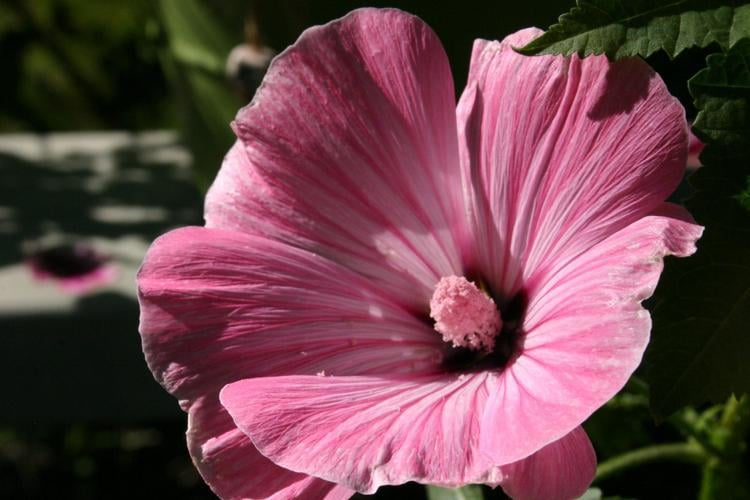
\includegraphics[width=0.14\textwidth,height=0.14\textwidth]{images/input_1.jpg} &
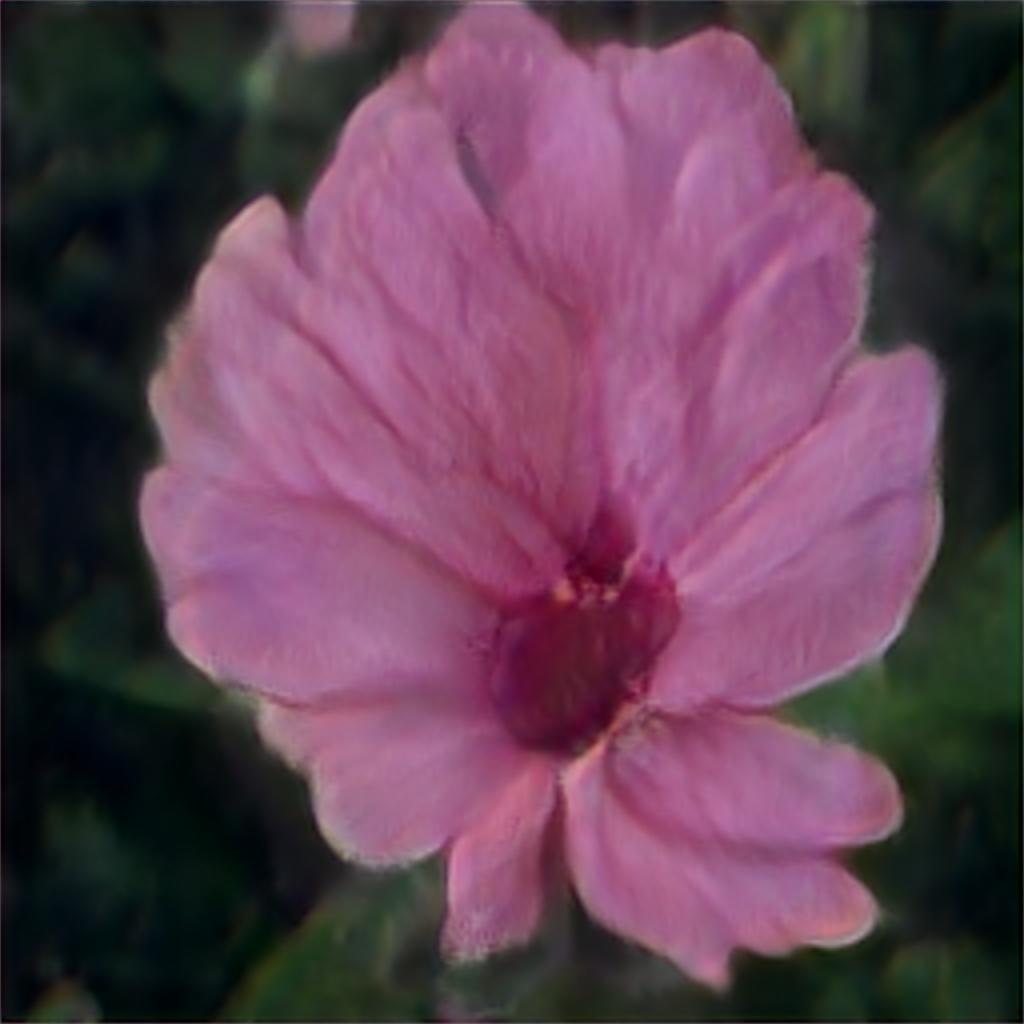
\includegraphics[width=0.14\textwidth,height=0.14\textwidth]{images/1age_output1.jpg} &
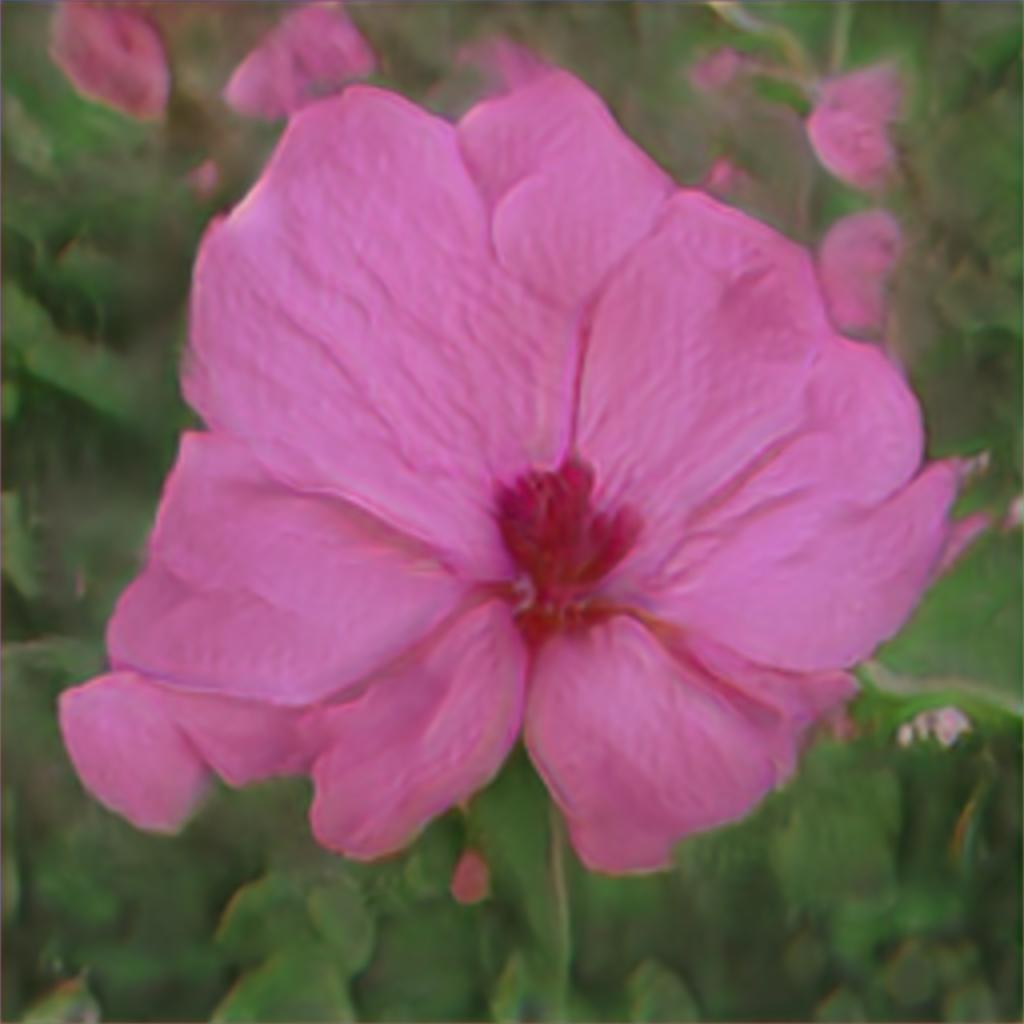
\includegraphics[width=0.14\textwidth,height=0.14\textwidth]{images/1age_output2.jpg} &
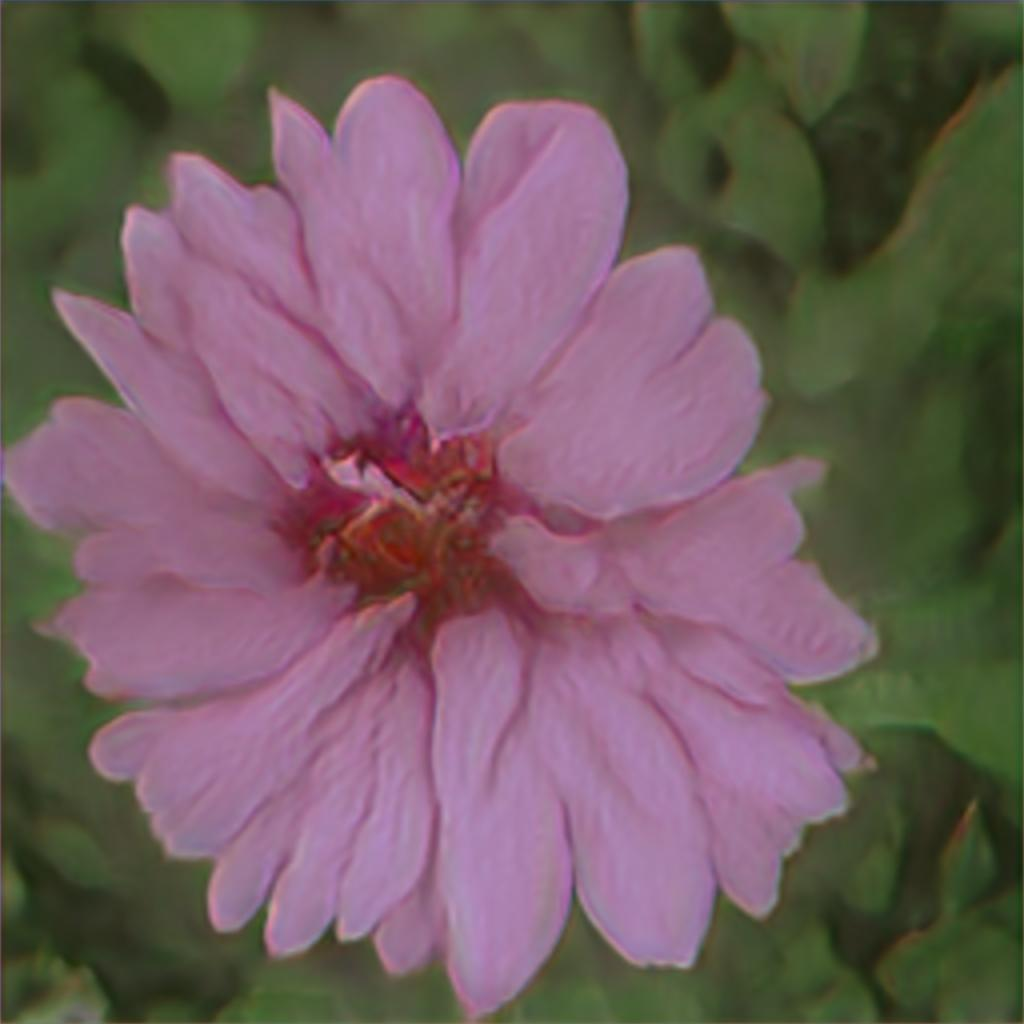
\includegraphics[width=0.14\textwidth,height=0.14\textwidth]{images/1sage_output1.jpg} &
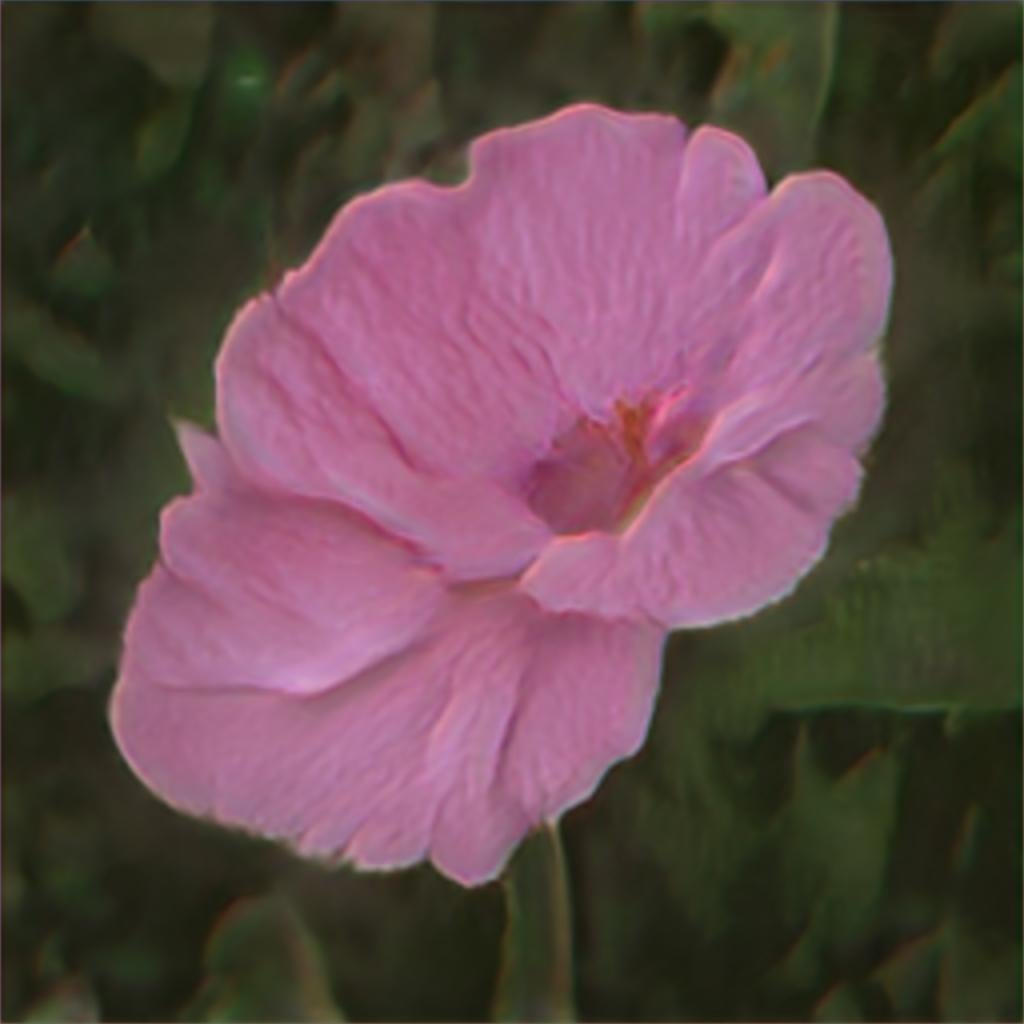
\includegraphics[width=0.14\textwidth,height=0.14\textwidth]{images/1sage_output2.jpg} &
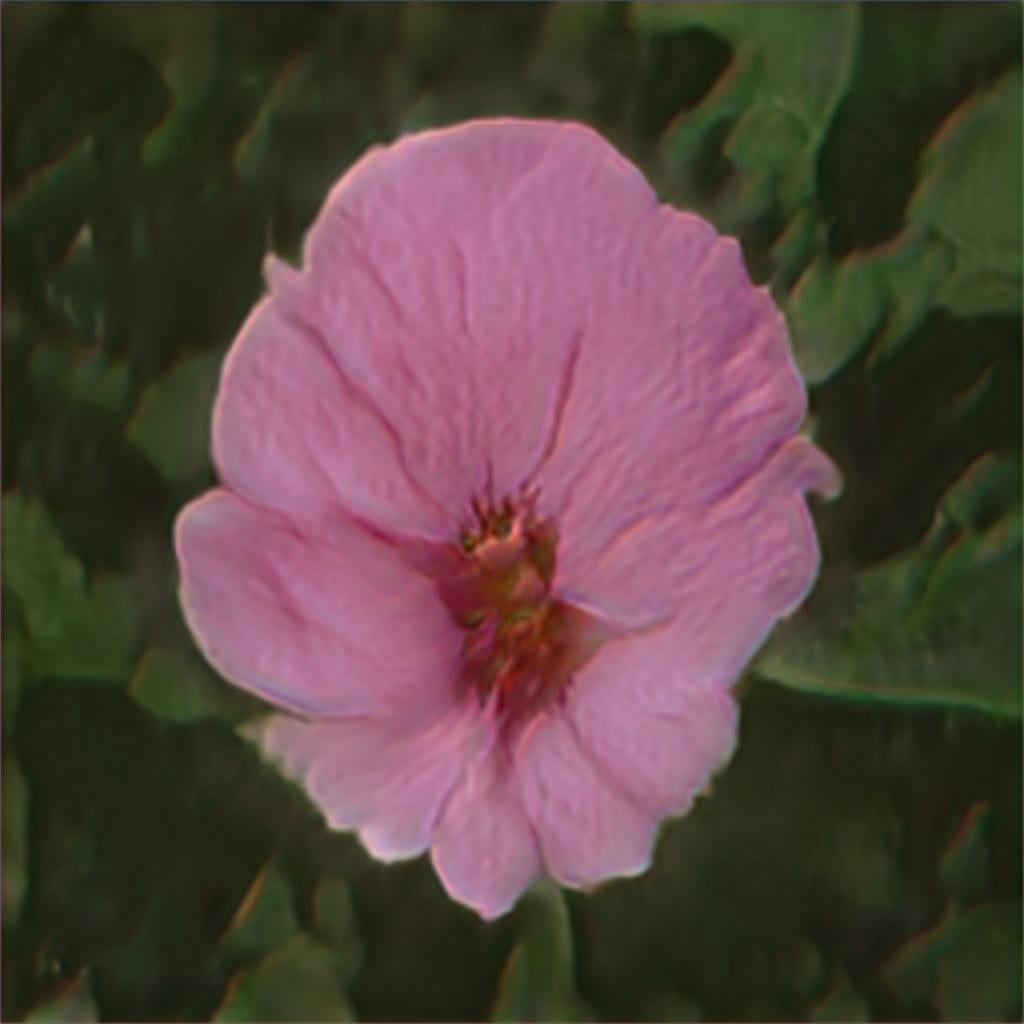
\includegraphics[width=0.14\textwidth,height=0.14\textwidth]{images/1sfsage_output1.jpg} &
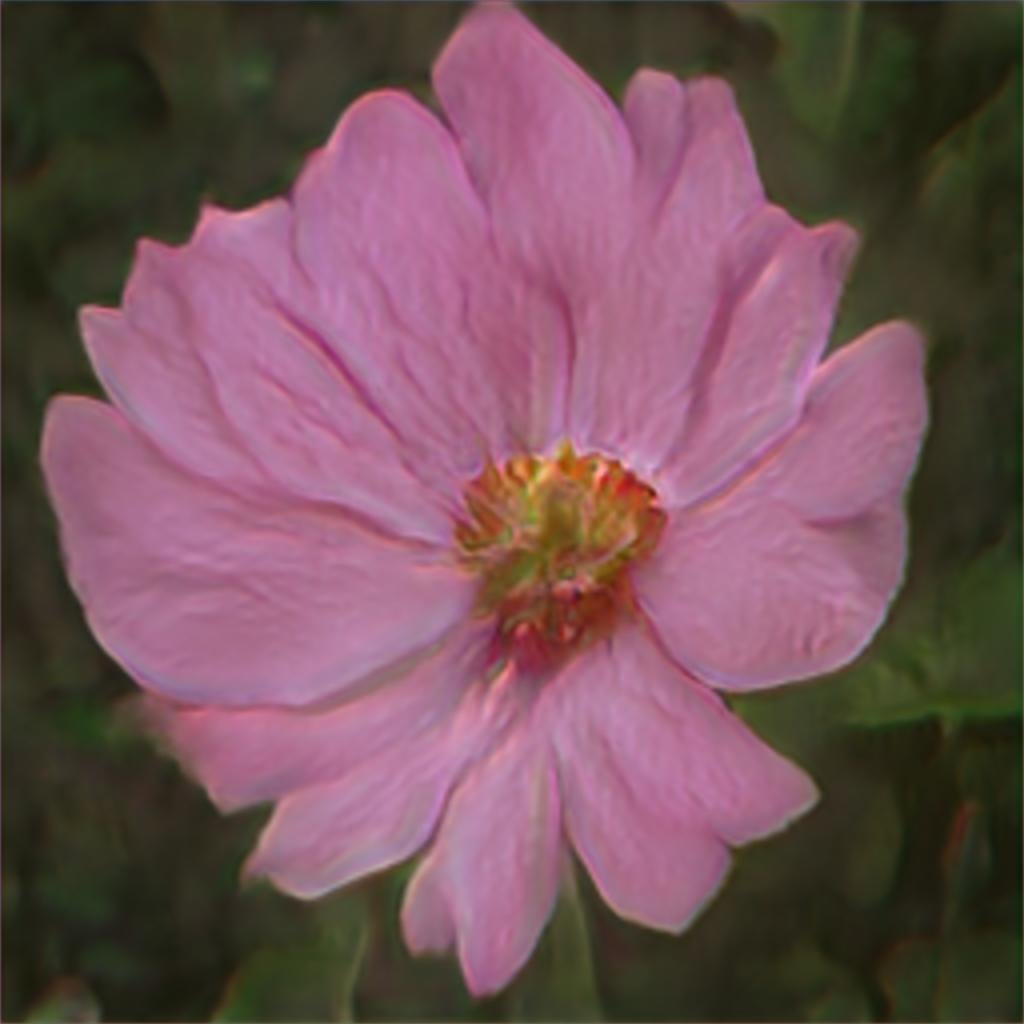
\includegraphics[width=0.14\textwidth,height=0.14\textwidth]{images/1sfsage_output2.jpg}
\\
Input & AGE & AGE & SAGE & SAGE & SFSAGE & SFSAGE
\end{tabular}

\caption{Comparison across AGE, SAGE, and the proposed SFSAGE model under one-shot setting, where a single reference image is used to condition the model during inference.}
\label{fig:qualitative_comparison}
\end{figure}


\begin{figure}[H]
\centering
\setlength{\tabcolsep}{2pt}

\begin{tabular}{ccccccc}
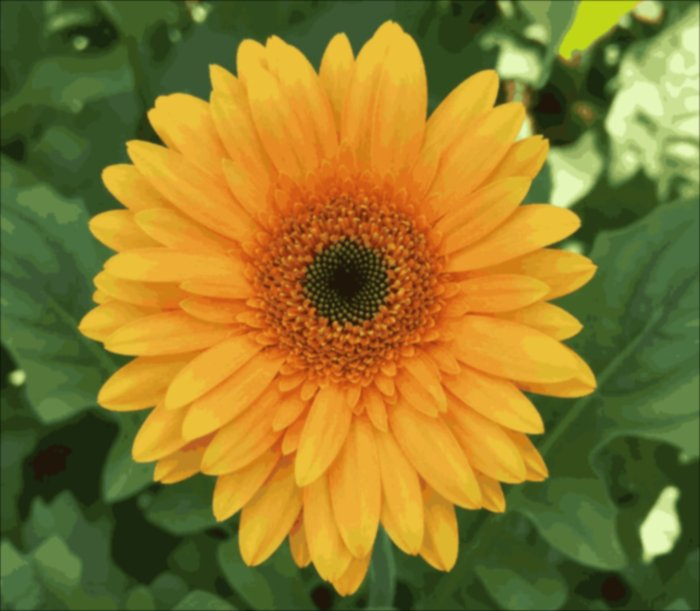
\includegraphics[width=0.14\textwidth,height=0.14\textwidth]{images/input_2.png} &
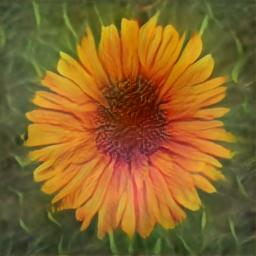
\includegraphics[width=0.14\textwidth,height=0.14\textwidth]{images/2age_output1.jpg} &
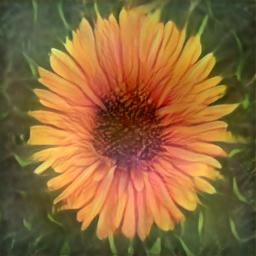
\includegraphics[width=0.14\textwidth,height=0.14\textwidth]{images/2age_output2.jpg} &
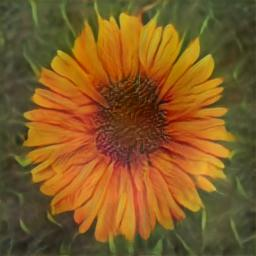
\includegraphics[width=0.14\textwidth,height=0.14\textwidth]{images/2sage_output1.jpg} &
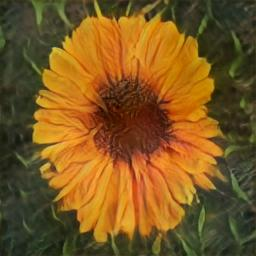
\includegraphics[width=0.14\textwidth,height=0.14\textwidth]{images/2sage_output2.jpg} &
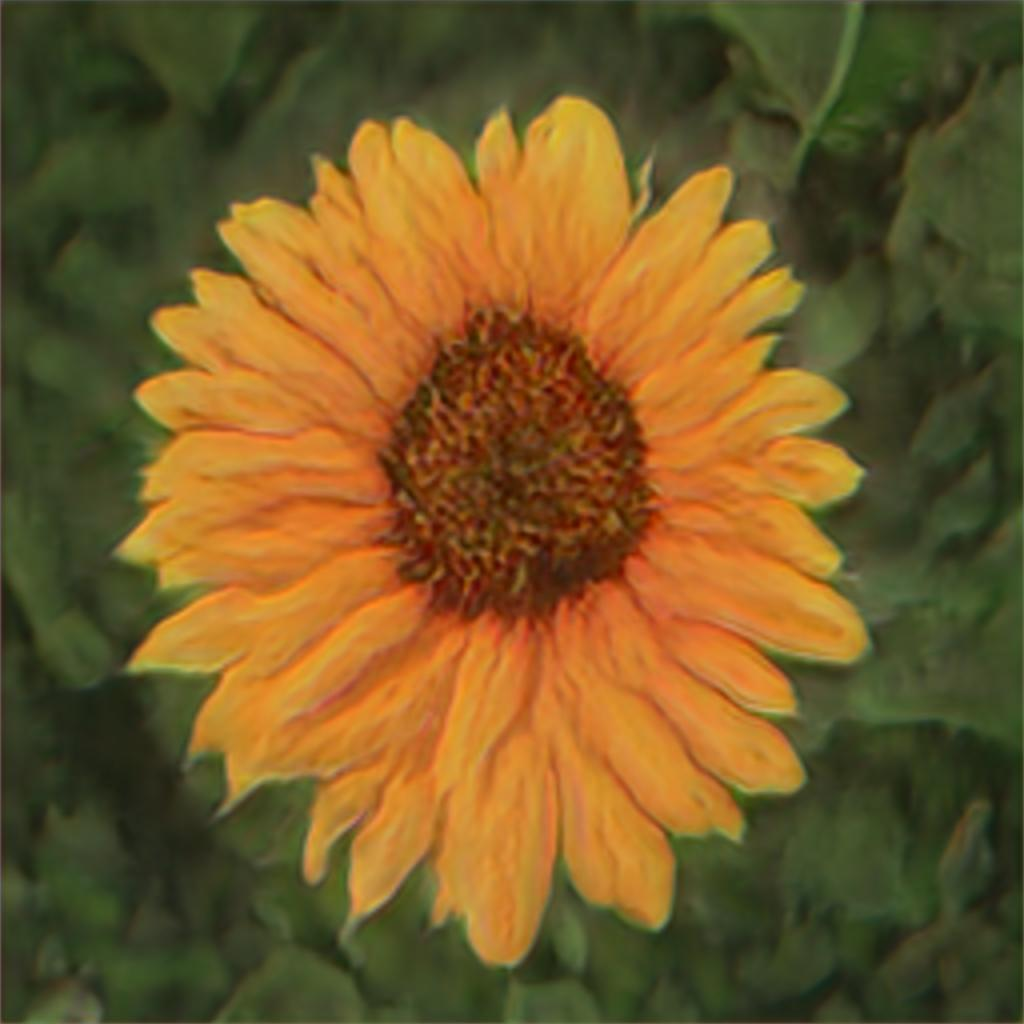
\includegraphics[width=0.14\textwidth,height=0.14\textwidth]{images/2sfsage_output1.jpg} &
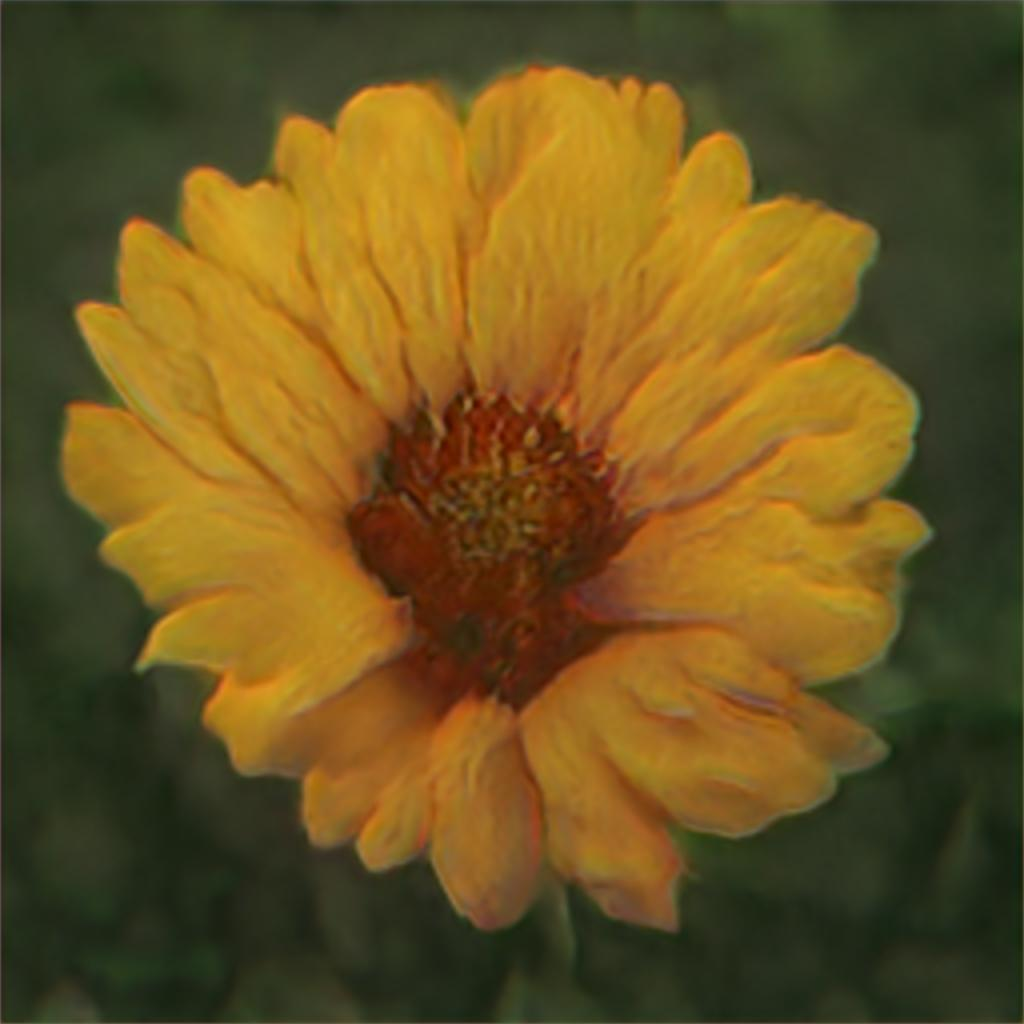
\includegraphics[width=0.14\textwidth,height=0.14\textwidth]{images/2sfsage_ouptut2.jpg}
\\
Input & AGE & AGE & SAGE & SAGE & SFSAGE & SFSAGE
\end{tabular}

\caption{Comparison across AGE, SAGE, and the proposed SFSAGE model under one-shot setting with a different image input.}
\label{fig:qualitative_input2}
\end{figure}

% image names for af:
% input3.png, age_af_output1.jpg, age_af_output2.jpg, sage_af_output1.jpg, sfsage_af_output1.jpg, sage_output2.jpg, sfsage_af_ouptut2.jpg

\begin{figure}[H]
\centering
\setlength{\tabcolsep}{2pt}

\begin{tabular}{ccccccc}
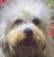
\includegraphics[width=0.14\textwidth,height=0.14\textwidth]{images/input3.jpg} &
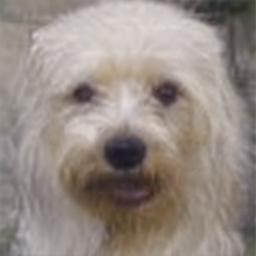
\includegraphics[width=0.14\textwidth,height=0.14\textwidth]{images/age_af_output1.jpg} &
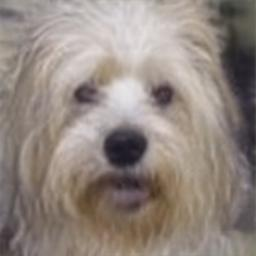
\includegraphics[width=0.14\textwidth,height=0.14\textwidth]{images/age_af_output2.jpg} &
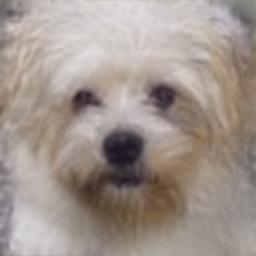
\includegraphics[width=0.14\textwidth,height=0.14\textwidth]{images/sage_af_output1.jpg} &
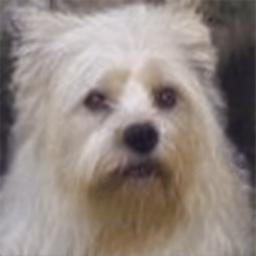
\includegraphics[width=0.14\textwidth,height=0.14\textwidth]{images/sage_output2.jpg} &
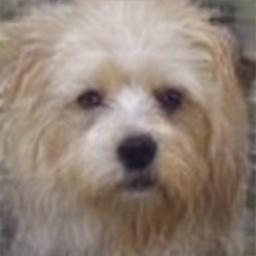
\includegraphics[width=0.14\textwidth,height=0.14\textwidth]{images/sfsage_af_output1.jpg} &
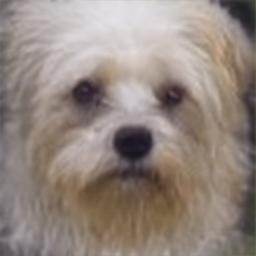
\includegraphics[width=0.14\textwidth,height=0.14\textwidth]{images/sfsage_af_ouptut2.jpg} \\
Input & AGE & AGE & SAGE & SAGE & SFSAGE & SFSAGE
\end{tabular}

\caption{Comparison across AGE, SAGE, and the proposed SFSAGE model on the Animal Faces dataset under one-shot setting. Each model generates two outputs per input image to demonstrate edit diversity and semantic consistency.}
\label{fig:qualitative_animalfaces}
\end{figure}


\subsection{Visual Observations}

\subsubsection{Flowers}

Figures \ref{fig:qualitative_comparison} and \ref{fig:qualitative_input2} describe the qualitative analysis of the results of the edited flowers 
based on the baseline models AGE and SAGE, and the proposed model SFSAGE. The models are compared with regard to their ability to maintain the 
colors properly, the sharpness of the images, the level of contrast, and realism. As shown in Figure \ref{fig:qualitative_comparison}, the proposed 
model performs well in the retention of the pink petal colors from the input images. It also performs much better based on the level of semantic 
consistency. Note that the proposed model also fails to represent the combined red and yellow colors of the pistil from the input images. On the 
other hand, the proposed model performs much better than both the input images in the sharpness of the petal. Although there are inconsistencies 
from the input images, the proposed model also performs much better. In addition, the level of contrast in the proposed model results in the sharpest 
flower among all the models. Further, the advantages of SFSAGE are highlighted by Figure \ref{fig:qualitative_input2}. The sharpness in petal edges 
is better retained by the model compared to AGE and SAGE, which allows for a more photo-realistic and organic rendering. More varied outputs have 
also resulted from SFSAGE; for instance, in one generated image, the flower is presented with a slight tilt, reflecting strong attribute manipulation. 
The model maintains higher clarity, with balanced contrast and natural color distribution, while AGE slightly looks pale with reduced contrast in 
areas, which is somewhat settled by SAGE as it balances the contrast. Overall, the 65 generated flower images produced by SFSAGE are the sharpest, 
most realistic, and visually consistent as compared to the other models being tested.

\subsubsection{Animal Faces}

Figure \ref{fig:qualitative_animalfaces} provides a comparison of the outputs produced by the AGE, SAGE, and proposed SFSAGE model on the 
Animal Faces data set using a picture of a dog as input. As observed, the outputs produced by the models have managed to maintain the color 
and texture of the input data, implying success by these models in maintaining basic characteristics produced by each model. Considering the 
clarity and image properties, all the outputs produced by these models can be considered similar, since there is minimal blurring effect and 
texture preservation on the fur of the input image. Consistency and overall properties, on the other hand, differ significantly, since there 
is more diversity apparent in the outputs produced by the AGE and SAGE models, with a slight difference in orientation between the two outcomes 
produced by each model. The more consistent results produced by the proposed SFSAGE model, on the contrary, demonstrate success towards 
maintaining integrity while providing semantic edits. Also, there are some minor enhancements in the realism of the output, whereby the output 
from SFSAGE shows slightly more coherent shading and blending of the fur patterns. This indicates that although all these models demonstrate 
the ability to sustain basic attributes like color and texture, the SFSAGE model has the best consistency in output.

\section{Failure Cases and Limitations}

During experimentation and evaluation of the FeatureSAGE framework, two main limitations were observed:

\begin{enumerate}
    \item \textbf{Dependence on a pretrained StyleGAN2 generator.} FeatureSAGE inherits the coverage and biases of the pretrained StyleGAN2 generator. If the generator does not adequately represent certain categories or visual attributes, those gaps may appear in the generated outputs. This constraint limits the framework to domains where an appropriate pretrained StyleGAN2 model is available and sufficiently aligned with the target data.

    \item \textbf{Computational overhead.} Integrating the StyleFeatureEditor inverter and Feature Editor increases the computational cost relative to the baseline SAGE setup. These components improve reconstruction and feature-level editing, but they require additional generator passes and feature-tensor operations. As a result, the framework requires more GPU memory and can slow inference or training, especially when scaling to larger datasets or time-sensitive applications.
\end{enumerate}

These limitations indicate that the reported quality improvements involve a trade-off between image fidelity and computational efficiency. They also motivate future work on lighter inversion modules, more efficient feature editing, and evaluation with generator backbones beyond StyleGAN2.
